%% LaTeX Template for ISIT 2018
%%
%% by Stefan M. Moser, October 2017
%%
%% derived from bare_conf.tex, V1.4a, 2014/09/17, by Michael Shell
%% for use with IEEEtran.cls version 1.8b or later
%%
%% Support sites for IEEEtran.cls:
%%
%% http://www.michaelshell.org/tex/ieeetran/
%% http://moser-isi.ethz.ch/manuals.html#eqlatex
%% http://www.ctan.org/tex-archive/macros/latex/contrib/IEEEtran/
%%

\documentclass[conference]{IEEEtran}


%%%%%%
%% Packages:
%% Some useful packages (and compatibility issues with the IEEE format)
%% are pointed out at the very end of this template source file (they are 
%% taken verbatim out of bare_conf.tex by Michael Shell).
%
% *** Do not adjust lengths that control margins, column widths, etc. ***
% *** Do not use packages that alter fonts (such as pslatex).         ***
%
\usepackage[utf8]{inputenc} 
\usepackage[T1]{fontenc}
\usepackage{url}
\usepackage{ifthen}
\usepackage{cite}
\usepackage[cmex10]{amsmath} % Use the [cmex10] option to ensure complicance
                             % with IEEE Xplore (see bare_conf.tex)

\usepackage[color=green!40,textsize=scriptsize]{todonotes}
\usepackage{amssymb}
\usepackage[colorlinks=true,allcolors=blue!90!green!90!red]{hyperref}
\usepackage{mathtools}
\mathtoolsset{showonlyrefs}

%% Please note that the amsthm package must not be loaded with
%% IEEEtran.cls because IEEEtran provides its own versions of
%% theorems. Also note that IEEEXplore does not accepts submissions
%% with hyperlinks, i.e., hyperref cannot be used.

\interdisplaylinepenalty=2500 % As explained in bare_conf.tex


%%%%%%
% correct bad hyphenation here
\hyphenation{op-tical net-works semi-conduc-tor}

% ------------------------------------------------------------

\begin{document}

\title{Solving Partial Differential Equations Using Convex Optimization}

%%% Single author, or several authors with same affiliation:
\author{%
  \IEEEauthorblockN{Nav Ravindranath}
  \IEEEauthorblockA{Columbia University\\
                    Applied Physics and Applied Mathematics\\
                    New York, NY\\
                    Email: ngr2114@columbia.edu}
}

%%% Several authors with up to three affiliations:
% \author{%
%   \IEEEauthorblockN{Stefan M.~Moser}
%   \IEEEauthorblockA{ETH Zürich\\
%                     ISI (D-ITET), ETH Zentrum\\
%                     CH-8092 Zürich, Switzerland\\
%                     Email: moser@isi.ee.ethz.ch}
%   \and
%   \IEEEauthorblockN{Albus Dumbledore and Harry Potter}
%   \IEEEauthorblockA{Hogwarts School of Witchcraft and Wizardry\\
%                     Hogwarts Castle\\
%                     1714 Hogsmeade, Scotland\\
%                     Email: \{dumbledore, potter\}@hogwarts.edu}
% }

%%% Many authors with many affiliations:
% \author{%
%   \IEEEauthorblockN{Albus Dumbledore\IEEEauthorrefmark{1},
%                     Olympe Maxime\IEEEauthorrefmark{2},
%                     Stefan M.~Moser\IEEEauthorrefmark{3}\IEEEauthorrefmark{4},
%                     and Harry Potter\IEEEauthorrefmark{1}}
%   \IEEEauthorblockA{\IEEEauthorrefmark{1}%
%                     Hogwarts School of Witchcraft and Wizardry,
%                     1714 Hogsmeade, Scotland,
%                     \{dumbledore, potter\}@hogwarts.edu}
%   \IEEEauthorblockA{\IEEEauthorrefmark{2}%
%                     Beauxbatons Academy of Magic,
%                     1290 Pyrénées, France,
%                     maxime@beauxbatons.edu}
%   \IEEEauthorblockA{\IEEEauthorrefmark{3}%
%                     ETH Zürich, ISI (D-ITET), ETH Zentrum, 
%                     CH-8092 Zürich, Switzerland,
%                     moser@isi.ee.ethz.ch}
%   \IEEEauthorblockA{\IEEEauthorrefmark{4}%
%                     National Chiao Tung University (NCTU), 
%                     Hsinchu, Taiwan,
%                     moser@isi.ee.ethz.ch}
% }

\maketitle


%%%%%%
%% Abstract:
%% If your paper is eligible for the student paper award, please add
%% the comment "THIS PAPER IS ELIGIBLE FOR THE STUDENT PAPER
%% AWARD." as a first line in the abstract.
%% For the final version of the accepted paper, please do not forget
%% to remove this comment!
%%
\begin{abstract}
  We present a method for solving partial differential equations (PDEs) using standard convex optimization tools, such as CVX \cite{cvx,gb08}. The proposed method provides a declarative syntax for specifying the PDE, thereby greatly simplifying the handling of boundary conditions. As a result, researchers implementing numerical methods not supported by existing solvers can quickly explore the effectiveness of a large number of numerical schemes on their problem before investing the time to implement the schemes using more traditional approaches, which may be required for computational efficiency reasons after increasing the resolution of the simulation. In addition to demonstrating how PDEs can be expressed as convex optimization problems, we explore the scalability limits of convex solvers in the context of PDEs.
\end{abstract}


\section{Introduction}

When modeling complicated physical phenomena such as atmospheric processes or tropical storms, the problem is often defined as a system of PDEs which need to be solved numerically. Unfortunately, standard off-the-shelf solvers for PDEs are usually inadequate for solving such problems. It is common for researchers to develop their own numerical PDE solvers which exploit special structure unique to their problem \todo{Cite}.

When developing a new PDE solver, there are several important aspects which need to be considered. First is the consistency of the numerical method, which is usually determined analytically. Next is the stability and convergence of the method. While theoretical guarantees can be given for many numerical methods regarding rates of convergence, the rates can sometimes be misleading in practice due to the sizes of constants on leading error terms, which can be problem dependent \todo{Cite}. Fortunately, the rate at which the accuracy of a simulation improves as the resolution of the simulation is increased can be observed for a specific problem experimentally. However, in order to do so, the numerical method first needs to be correctly implemented.

One of the trickiest aspects of implementing numerical solvers for PDEs is correctly incorporating boundary conditions into the numerical scheme \todo{Cite}. For illustration, we start by considering a simple example -- a finite difference method for Poisson's equation in 2 dimensions. Poisson's equation takes the form
\begin{equation}
  \nabla^2 u = f
\end{equation}
where $\nabla^2 u = u_{xx} + u_{yy}$ in 2 dimensions. In order for the problem to be well posed, we also need conditions to be specified at the boundaries of the domain. For simplicity, we consider the Dirichlet boundary conditions
\begin{align}
  u(0, y) &= g_0(y) \\
  u(M, y) &= g_1(y) \\
  u(x, 0) &= h_0(x) \\
  u(x, N) &= h_1(x)
\end{align}
on a rectangular domain of size $M \times N$.

Suppose we discretize the domain using $m$ interior points in the $x$-direction and $n$ interior points in the $y$-direction, uniformly spaced in each direction, so that we have a mesh of size $(m+2) \times (n+2)$ consisting of the points $\{(x_i, y_j)\}$ where $i \in \{0,\ldots,m+1\}, j \in \{0,\ldots,n+1\}$ with the boundaries included. The discretized solution $U$ consists of the values of the continuous solution $u$ on the grid points of the mesh. We similarly discretize the source term $f$ as an $(m+2) \times (n+2)$ matrix $F$. It remains to discretize the Laplacian operator $\nabla^2$.

A common discrete approximation to the Laplacian is the 5-point discrete Laplacian operator given by \todo{Cite}
\begin{equation}
  \nabla_5^2 U_{i,j} = \frac{U_{i-1,j} - 2U_{i,j} + U_{i+1,j}}{\Delta x^2} + \frac{U_{i,j-1} - 2U_{i,j} + U_{i,j+1}}{\Delta y^2}
\end{equation}
where $U_{i,j} = u(x_i, y_j), i \in \{0,\ldots,m+1\}, j \in \{0,\ldots,n+1\}$, and the mesh sizes in each direction are $\Delta x = (m+1)/M,$ and $\Delta y = (n+1)/N$. The 5-point discrete Laplacian operator is a second-order centered approximation to its continuous analogue.

As a step toward expressing the discretized equation as a convex optimization problem, we would like to write the discretized equation in matrix form. To do so, we construct the unrolled vectors
\begin{equation}
  \vec{U} = \begin{bmatrix}
    U_{0,0} \\ \vdots \\ U_{m+1,0} \\ \vdots \\ U_{0,n+1} \\ \vdots \\ U_{m+1,n+1}
  \end{bmatrix}, \quad \vec{F} = \begin{bmatrix}
    F_{0,0} \\ \vdots \\ F_{m+1,0} \\ \vdots \\ F_{0,n+1} \\ \vdots \\ F_{m+1,n+1}
  \end{bmatrix}
\end{equation}
with $F_{i,j}$ defined analogously to $U_{i,j}$. We can now express the discrete Laplacian $\nabla_5^2$ as a matrix of the form shown in Figure \ref{fig:discrete-laplacian}
\begin{figure}[t]
  \begin{center}
    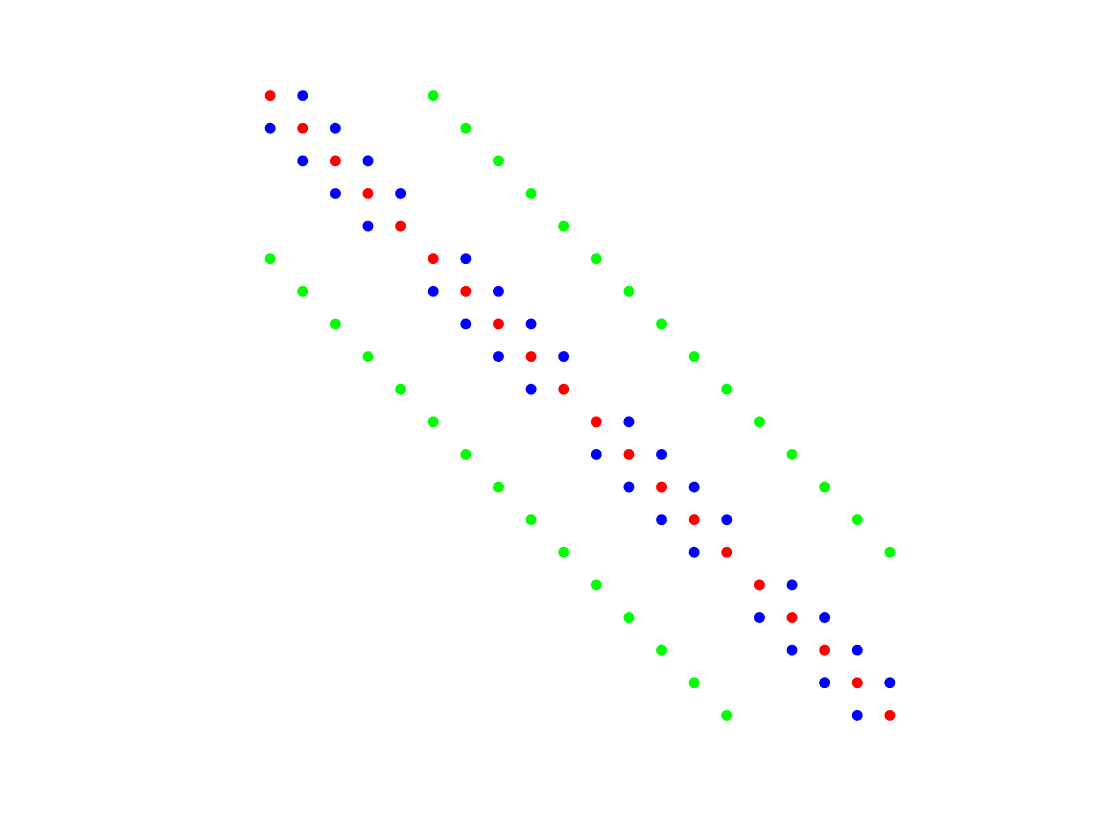
\includegraphics[width=0.48\textwidth]{figures/discrete-laplacian}
    \caption{Second-order centered discrete Laplacian matrix}
    \label{fig:discrete-laplacian}
  \end{center}
\end{figure}
where the entries on the main diagonal (indicated in red) take the value $-\frac{2}{\Delta x^2}-\frac{2}{\Delta y^2}$, the entries on the subdiagonal and superdiagonal (indicated in blue) take the value $\frac{1}{\Delta x^2}$, and the entries on the outer diagonals (indicated in green) take the value $\frac{1}{\Delta y^2}$.

Note that the off-diagonals have missing entries corresponding to the boundary points. Traditional methods of implementing numerical PDE solvers require adjusting for the missing entries either by using ghost cells \todo{Cite} or by modifying the discretized source term $F$ \todo{Cite}. As the PDE and choice of discretization become more complicated, correctly incorporating boundary conditions becomes increasingly cumbersome and significantly hinders the ability to quickly explore the effectiveness of hand-crafted numerical schemes for solving PDEs.


\section{Problem Formulation}

\subsection{Poisson's Equation}

The discrete version of Poisson's equation on the interior of the domain can now be expressed as
\begin{equation}
  (A_* \vec{U})^\circ = (\vec{F})^\circ
\end{equation}
where $A_*$ is the discrete Laplacian matrix shown in Figure \ref{fig:discrete-laplacian}, and ${}^\circ : \mathbb{R}^{(m+2)(n+2)} \to \mathbb{R}^{mn}$ is the operator defined by
\begin{equation}
  \begin{bmatrix}
    V_{0,0} \\ \vdots \\ V_{m+1,0} \\ \vdots \\ V_{0,n+1} \\ \vdots \\ V_{m+1,n+1}
  \end{bmatrix}^\circ = \begin{bmatrix}
    V_{1,1} \\ \vdots \\ V_{m,1} \\ \vdots \\ V_{1,n} \\ \vdots \\ V_{m,n}
  \end{bmatrix}
\end{equation}
that extracts the entries on the interior of the mesh. The Dirichlet boundary conditions can be easily imposed on the discretized solution as
\begin{align}
  U_{0,j} &= g_0(y_j) \\
  U_{m+1,j} &= g_1(y_j) \\
  U_{i,0} &= h_0(x_i) \\
  U_{i,n+1} &= h_1(x_i)
\end{align}
for $i \in \{0,\ldots,m+1\}$ and $j \in \{0,\ldots,n+1\}$.

Observe that the rows of $A_*$ with missing entries do not affect the result of $(A_* \vec{U})^\circ$. Therefore, we can simplify the structure of the discrete Laplacian matrix by filling in the missing entries as shown in Figure \ref{fig:modified-discrete-laplacian}.
\begin{figure}[t]
  \begin{center}
    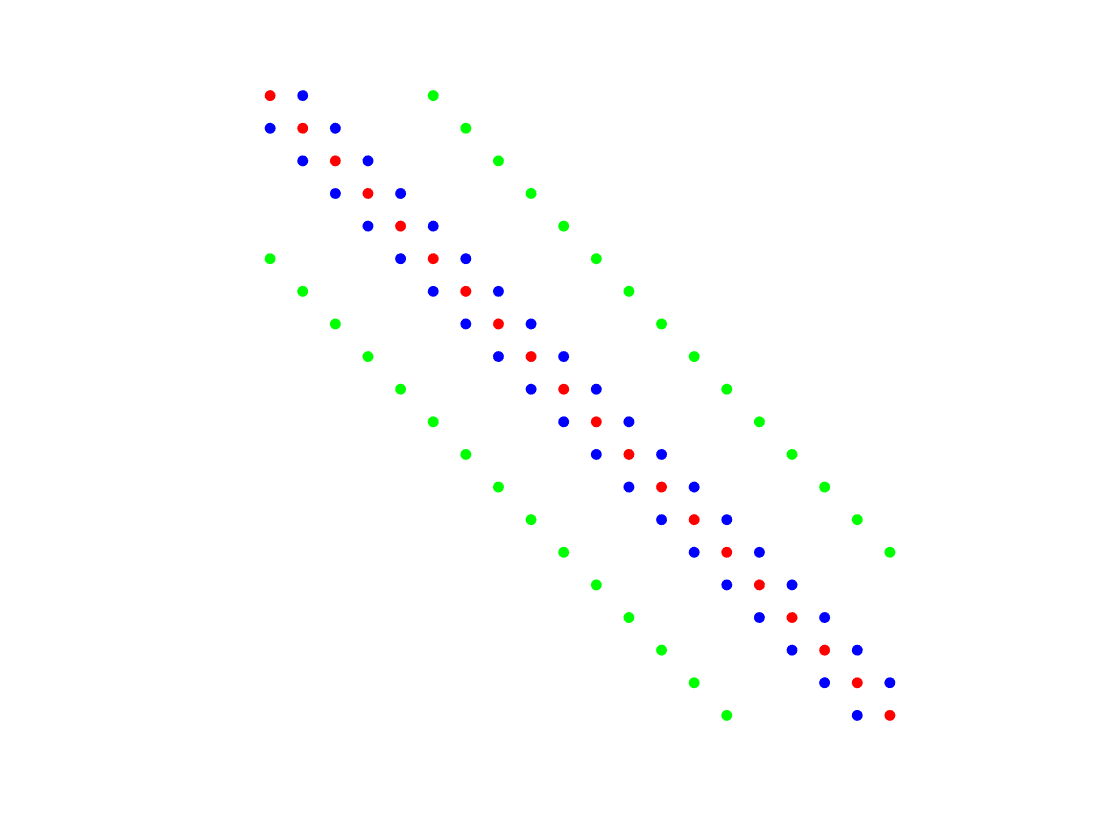
\includegraphics[width=0.48\textwidth]{figures/modified-discrete-laplacian}
    \caption{Modified second-order centered discrete Laplacian matrix}
    \label{fig:modified-discrete-laplacian}
  \end{center}
\end{figure}
In other words, if we let $A$ denote the matrix shown in Figure \ref{fig:modified-discrete-laplacian}, then we have
\begin{equation}
  (A_* \vec{U})^\circ = (A \vec{U})^\circ
\end{equation}
so that numerically solving for $U$ is equivalent to solving the convex optimization problem
\begin{equation}
  \begin{array}{lll}
    \text{minimize} & \|(A \vec{U} - \vec{F})^\circ\|_2 \\
    \text{subject to} & U_{0,j} = g_0(y_j), & j = 0,\ldots,n+1 \\
    & U_{m+1,j} = g_1(y_j), & j = 0,\ldots,n+1 \\
    & U_{i,0} = h_0(x_i), & i = 0,\ldots,m+1 \\
    & U_{i,n+1} = h_1(x_i), & i = 0,\ldots,m+1
  \end{array}
\end{equation}
where we minimize the norm of the difference between the left-hand and right-hand sides of the PDE, and impose the boundary conditions as constraints. The convex optimization problem is equivalent to a linearly constrained least squares problem upon squaring the objective function, since ${}^\circ$ is a linear operator.

\subsection{Heat Equation}

We now turn to a slightly more complicated PDE---the 2-dimensional heat equation---which adds an element of time to Poisson's equation. We consider the PDE
\begin{equation}
  \nabla^2 u = u_t
\end{equation}
with boundary conditions
\begin{align}
  u(0, y, t) &= g_0(y, t) \\
  u(M, y, t) &= g_1(y, t) \\
  u(x, 0, t) &= h_0(x, t) \\
  u(x, N, t) &= h_1(x, t)
\end{align}
and initial condition
\begin{equation}
  u(x, y, 0) = u_0(x, y)
\end{equation}
where $0 \le t \le T$. Furthermore, we discretize time into $p+1$ equispaced points between $0$ and $T$ (inclusive) with time step $\Delta t = T/p$. The discrete solution $U$ is now a 3-dimensional array over an $(m+2) \times (n+2) \times (p+1)$ grid with the value corresponding to $u(x_i, y_j, t_k)$ denoted by $U_{i,j}^k$ for $i \in \{0,\ldots,m+1\}, j \in \{0,\ldots,n+1\}, k \in \{0,\ldots,p\}$.

In order to convert the heat equation into matrix form, we define
\begin{equation}
  \vec{U}^k = \begin{bmatrix}
    U_{0,0}^k \\ \vdots \\ U_{m+1,0}^k \\ \vdots \\ U_{0,n+1}^k \\ \vdots \\ U_{m+1,n+1}^k
  \end{bmatrix}
\end{equation}
and
\begin{equation}
  \widetilde{U}_+ = \begin{bmatrix}
    \vec{U}^1 & \cdots & \vec{U}^p
  \end{bmatrix}, \quad \widetilde{U}_- = \begin{bmatrix}
    \vec{U}^0 & \cdots & \vec{U}^{p-1}
  \end{bmatrix}
\end{equation}
so that the discretized heat equation becomes
\begin{equation}
  \left(\frac{A(\widetilde{U}_+ + \widetilde{U}_-)}{2}\right)^\circ = \left(\frac{\widetilde{U}_+ - \widetilde{U}_-}{\Delta t}\right)^\circ
\end{equation}
using the Crank-Nicolson method \todo{Cite}, where the ${}^\circ$ operator is applied column-wise. Note that applying ${}^\circ$ is equivalent to left multiplication by the identity matrix with rows corresponding to boundary points removed. We can then express the heat equation as the convex optimization problem
\begin{equation}
  \begin{array}{lll}
    \text{minimize} & \left\|\left(\frac{A(\widetilde{U}_+ + \widetilde{U}_-)}{2} - \frac{\widetilde{U}_+ - \widetilde{U}_-}{\Delta t}\right)^\circ\right\|_F \\
    \text{subject to} & U_{0,j}^k = g_0(y_j, t_k) \\
    & U_{m+1,j}^k = g_1(y_j, t_k) \\
    & U_{i,0}^k = h_0(x_i, t_k) \\
    & U_{i,n+1}^k = h_1(x_i, t_k) \\
    & U_{i,j}^0 = u_0(x_i, y_j)
  \end{array}
\end{equation}
with the boundary conditions and initial condition as constraints, where $i$, $j$, and $k$ range over their possible values, and $\|\cdot\|_F$ denotes the Frobenius norm. Since the Frobenius norm can be expressed as a Euclidean vector norm, this problem is also equivalent to a linearly constrained least squares problem.


\section{Solutions}

Because the convex optimization problems described above will be solved by CVX using a conic solver, we minimize the norm of the residual rather than the squared norm \todo{Cite}. Specifying the convex optimization problem for Poisson's equation in CVX is straightforward; we construct the mesh from uniformly spaced vectors of grid points, evaluate the source term $f$ on the mesh, build the diagonal matrix $A$, and then specify the objective function and constraints almost exactly as stated in mathematical form.

Table \ref{tab:poisson-operators} shows how each of the mathematical operators in the objective function for Poisson's equation can be implemented in MATLAB\textsuperscript{\textregistered} \todo{Cite} with CVX. In Table \ref{tab:poisson-operators}, $X$ is an $(m+2) \times (n+2)$ matrix, $\vec{X}$ is the corresponding unrolled vector, and \texttt{X} is an $(m+2) \times (n+2)$ MATLAB\textsuperscript{\textregistered} array; $\vec{Y}$ is an $mn$-vector, and \texttt{Y} is the corresponding $mn \times 1$ MATLAB\textsuperscript{\textregistered} array.
\begin{table}[h]
  \renewcommand*{\arraystretch}{1.5}
  \begin{center}
    \caption{Implementation of operators in MATLAB\textsuperscript{\textregistered} with CVX for Poisson's equation}
    \label{tab:poisson-operators}
    \begin{tabular}{|c|c|}
      \hline
      \textbf{Mathematics} & \textbf{MATLAB\textsuperscript{\textregistered}} \\ \hline
      $\vec{X}$ & \texttt{X(:)} \\ \hline
      $(\vec{X})^\circ$ & \texttt{reshape(X(2:end-1,2:end-1), [], 1)} \\ \hline
      $\|\vec{Y}\|_2$ & \texttt{norm(Y)} \\ \hline
   \end{tabular}
  \end{center}
\end{table}

The solution to Poisson's equation computed by CVX on a $40 \times 25$ grid with source function
\begin{equation}
  f(x, y) = -2 \sin x \cos y
\end{equation}
and boundary conditions
\begin{align}
  u(0, y) &= u(3\pi, y) = 0 \\
  u(x, 0) &= u(x, 2\pi) = \sin x
\end{align}
is indicated in Figure \ref{fig:poisson-solution}.
\begin{figure}[b]
  \begin{center}
    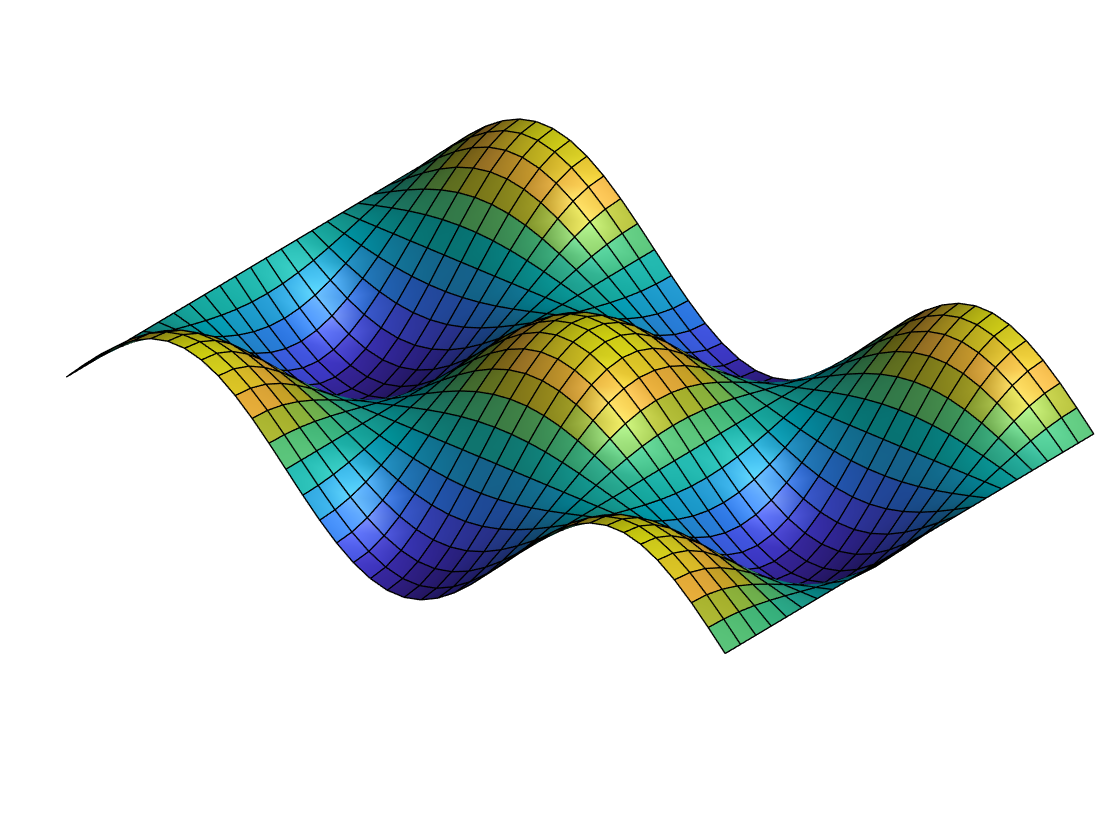
\includegraphics[width=0.48\textwidth]{figures/poisson-solution}
    \caption{Solution to Poisson's equation using CVX}
    \label{fig:poisson-solution}
  \end{center}
\end{figure}
The computed solution satisfies the boundary conditions and matches the analytical solution
\begin{equation}
  u(x, y) = \sin x \cos y
\end{equation}
as can be verified visually.

Solving the heat equation using CVX follows a similar procedure, except that we must work with 3-dimensional arrays rather than 2-dimensional ones, and additionally specify the initial condition as a constraint. Table \ref{tab:heat-operators} shows how the necessary operations can be performed in MATLAB\textsuperscript{\textregistered}. In the table below, \texttt{U} is an $(m+2) \times (n+2) \times (p+1)$ MATLAB\textsuperscript{\textregistered} array corresponding to the discrete solution $U$, and $V$ and $W$ are $(m+2)(n+2) \times p$ and $mn \times p$ matrices, respectively, with \texttt{V} and \texttt{W} as their MATLAB\textsuperscript{\textregistered} counterparts.
\begin{table}[h]
  \renewcommand*{\arraystretch}{1.5}
  \begin{center}
    \caption{Implementation of operators in MATLAB\textsuperscript{\textregistered} with CVX for heat equation}
    \label{tab:heat-operators}
    \begin{tabular}{|c|c|}
      \hline
      \textbf{Mathematics} & \textbf{MATLAB\textsuperscript{\textregistered}} \\ \hline
      $\widetilde{U}_+$ & \texttt{reshape(U(:,:,2:end), [], p)} \\ \hline
      $\widetilde{U}_-$ & \texttt{reshape(U(:,:,1:end-1), [], p)} \\ \hline
      & \texttt{tmp = reshape(V, m+2, n+2, p);} \\
      $V^\circ$ & \texttt{reshape(tmp(2:end-1,2:end-1,:), [], p)} \\ \hline
      $\|W\|_F$ & \texttt{norm(W(:))} \\ \hline
   \end{tabular}
  \end{center}
\end{table}

Figure \ref{fig:heat-solution} shows snapshots of the solution computed by CVX on a $40 \times 25 \times 17$ grid with $T = 1.6$, boundary conditions
\begin{align}
  u(0, y, t) &= u(3\pi, y, t) = 0 \\
  u(x, 0, t) &= u(x, 2\pi, t) = \sin x
\end{align}
and initial condition
\begin{align}
  u_0(x, y) = \sin x \cos y
\end{align}
which was the solution to Poisson's equation from before on the same spatial domain.
\begin{figure}[b]
  \begin{center}
    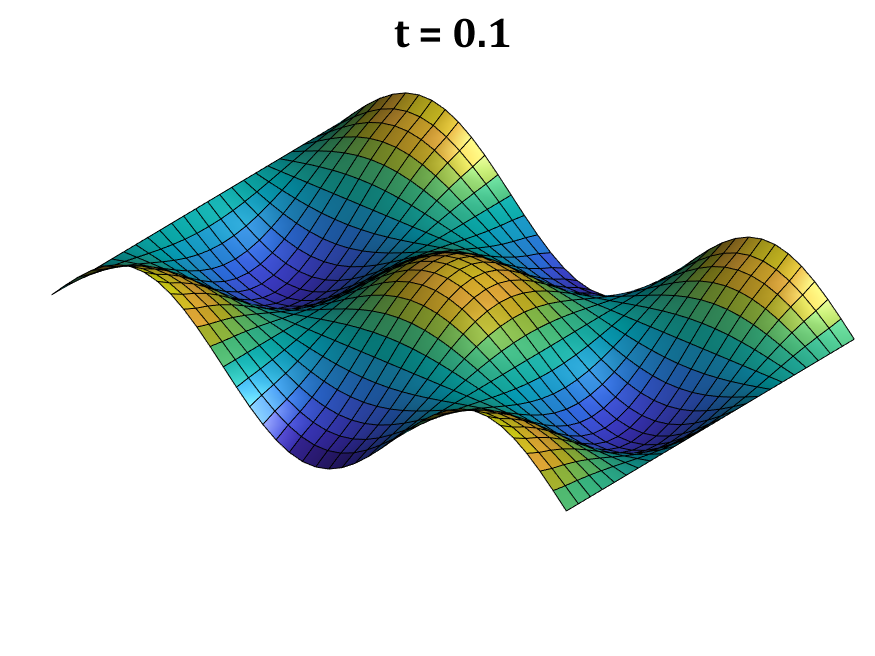
\includegraphics[width=0.24\textwidth,trim={1cm 1cm 0 0},clip]{figures/heat-solution-1}
    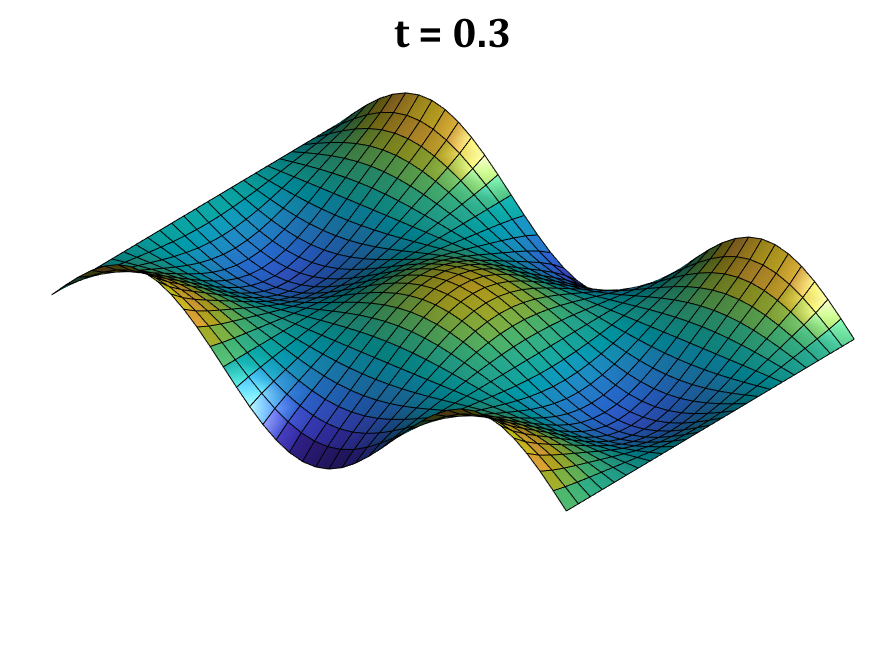
\includegraphics[width=0.24\textwidth,trim={1cm 1cm 0 0},clip]{figures/heat-solution-3}
    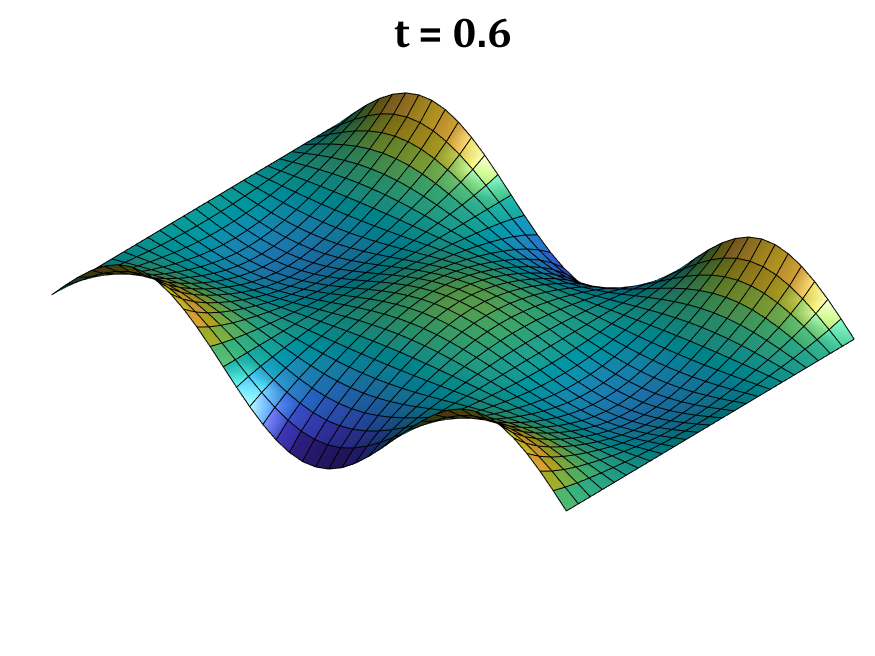
\includegraphics[width=0.24\textwidth,trim={1cm 1cm 0 0},clip]{figures/heat-solution-6}
    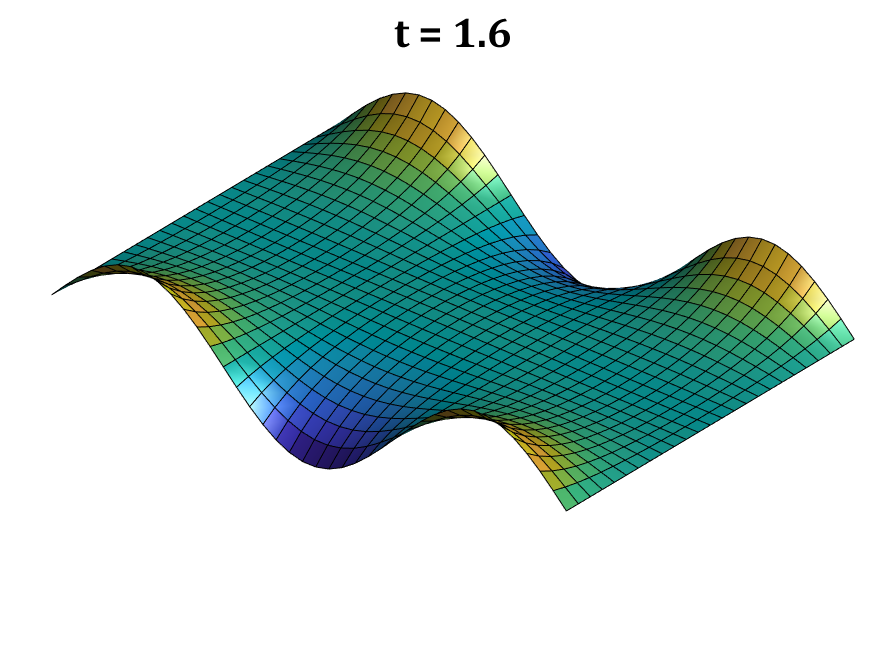
\includegraphics[width=0.24\textwidth,trim={1cm 1cm 0 0},clip]{figures/heat-solution-16}
    \caption{Solution to heat equation using CVX}
    \label{fig:heat-solution}
  \end{center}
\end{figure}
As expected, the initial heat distribution diffuses away while maintaining the boundary conditions \todo{Cite}.


\section{Analysis}

We now examine how the computational time required for CVX to solve the PDEs scales as the mesh is made finer. First, we increasingly refine the spatial grid by a factor of 2 in each dimension and observe the effect on the time required to solve Poisson's equation using CVX. Figure \ref{fig:poisson-scale} 
\begin{figure}[h]
  \begin{center}
    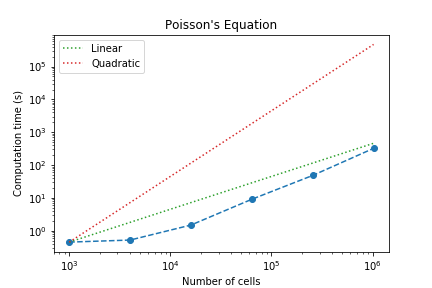
\includegraphics[width=0.48\textwidth]{figures/poisson-scale}
    \caption{Scaling of computation time with respect to spatial refinement}
    \label{fig:poisson-scale}
  \end{center}
\end{figure}
indicates that the computation time grows faster than linearly but slower than quadratically with the number of grid points. The finest mesh consisted of 1,024,000 grid points and took 322.97 seconds to solve with an Intel\textsuperscript{\textregistered} Core\texttrademark{} i7-6820HQ processor at 2.70 GHz and 32 GB RAM.

Next, we consider how the time required to solve the heat equation changes as we increase the number of time steps while keeping the initial and final times fixed. Figure \ref{fig:heat-scale}
\begin{figure}[h]
  \begin{center}
    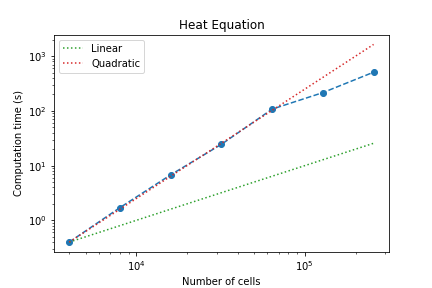
\includegraphics[width=0.48\textwidth]{figures/heat-scale}
    \caption{Scaling of computation time with respect to temporal refinement}
    \label{fig:heat-scale}
  \end{center}
\end{figure}
shows that the computation time grows quadratically with the number of grid points. For the finest mesh, we used 256,000 grid points, which required 509.70 seconds to solve.


\section{Conclusion}

Expressing a PDE as a convex optimization problem is an effective way to test how a numerical method performs on the PDE without having to explicitly implement the intricacies of the numerical scheme. We've seen how convex optimization provides a powerful declarative syntax to specify a discretization of a PDE along with its boundary and initial conditions without having to use techniques such as ghost cells or source term modification to embed boundary conditions into the discretization. In some cases, we can even additionally simplify the problem, for example, by conveniently filling in missing entries in the discrete Laplacian.

Furthermore, we observed experimentally that the time required to solve PDEs using CVX only grows quadratically with the number of grid points, enabling convergence studies to be performed as the mesh is refined for moderately sized problems. For larger problems, expressing a PDE as a convex optimization problem provides the potential to leverage existing distributed convex solvers without having to write custom distributed PDE solvers, as they can be error-prone and time-consuming to implement.

Finally, having a declarative syntax to specify a numerical method for solving PDEs reduces the chance of introducing bugs in the solver and provides a reference implementation for comparison if a more efficient custom solver is later written.


\section*{Notes}

The MATLAB\textsuperscript{\textregistered} code used to solve Poisson's equation and the heat equation, along with the code to generate the figures in this paper, is available at \url{https://github.com/navravi/eeor4650-project}.

\todo[inline]{Upload code to GitHub}


%%%%%%
%% To balance the columns at the last page of the paper use this
%% command:
%%
%\enlargethispage{-1.2cm}
%%
%% If the balancing should occur in the middle of the references, use
%% the following trigger:
%%
%\IEEEtriggeratref{3}
%%
%% which triggers a \newpage (i.e., new column) just before the given
%% reference number. Note that you need to adapt this if you modify
%% the paper.  The "triggered" command can be changed if desired:
%%
%\IEEEtriggercmd{\enlargethispage{-20cm}}
%%
%%%%%%

%%%%%%
%% References:
%% We recommend the usage of BibTeX:
%%
\bibliographystyle{IEEEtran}
\bibliography{bibliofile}
%%
%% BibTeX documentation can be obtained at:
%% http://www.ctan.org/tex-archive/biblio/bibtex/contrib/doc/
%%%%%%


\end{document}
